%Sample uscthesis, by Jose M Vidal
%Use PDFLaTeX to compile this since the Graduate school wants a pdf file.
%latex->dvi->ps->pdf also works, but is just silly.

%Some packages, such as float.sty and algorithm.sty, have to be loaded
%before uscthesis. In general, load uscthesis last.
\documentclass[12pt]{report}
\usepackage{latexsym}
\usepackage{amsmath}
\usepackage{indentfirst}
\usepackage[pdftex]{graphicx}
\usepackage{floatflt}
\usepackage{uscthesis}
%To get single-space, (for drafts only!) use:
%\singlespacing

\title{Multiple Input Transfer Function Modelling for Streamflow Data}
\author{Samuel Timothy Croker}

\abstract{ Developing a working multiple input transfer function
model of streamflow data is a difficult task due both to the
natural processes that generate the data and because of the
inaccuracies of the data collection process.  Still, much useful
information can be gathered from applying ARIMA transfer function
modelling to small, representative time periods.  It is possible
to develop reasonably well-behaved and accurate models even while
seriously limiting the amount of data cleaning that is done.}

%Degree you are applying for, defaults to Master of Engineering
\degree{Master of Science}
%\degree{Doctor of Philosophy}

%Your Previous Degree \\ University, year
\authordegree{Bachelor of Science \\ University of South Carolina, 1999}

%Example with two degrees:
%\authordegree{Master of Arts \\ University of South Carolina, 1922
%  \\ \vspace{1em}
%Bachelor of Arts\\ University of South Carolina, 1919}

%Students' college defaults to COE&IT.
\college{Science and Mathematics}

%All departments default to Computer Science and Engineering, but you can
%change them.
%Student's dept
\dept{Statistics} \directordept{Statistics}
\secondreaderdept{Statistics} \thirdreaderdept{Statistics}

%Year thesis is submitted
\copyrightyear{2005}

\begin{document}

%For MS students
\makethesistitle

%For PhD students
%\makedissertationtitle

%PhD only, and then only if you elect to Copyright your dissertation
%\makecopyrightpage

%Optional
%\prefacesection{Acknowledgments}
%I would like to thank my advisor for allowing me to graduate.

%For PhD dissertations. This abstract conforms to the UMI guidelines.
%The abstract must be 350 words or less.
%\director{Dr. Lousy Advisor}
%\makeumiabstract

%For MS thesis (or, you can use the one for PhD). This abstract
%maintains the same look as all other sections.
\makeabstract

%Optional
%\prefacesection{Preface}

\tableofcontents

%Uncomment following line if you have 4 or more tables
\makelistoftables

%Uncomment following line if you have 4 or more figures
\makelistoffigures

%Optional
%\prefacesection{List of Abbreviations}

%Start numbering in arabic
\pagenumbering{arabic}


\chapter{Introduction}
 The Congaree River is
formed by the confluence of the Saluda and Broad Rivers near
Columbia, SC.  Both the Saluda and the Broad Rivers are dam
controlled with the Saluda being managed by the Lake Murray Dam 7
miles above the Congaree, and the Broad managed by Parr Shoals Dam
which is about 20 miles above the confluence of the two rivers.
\begin{figure}[h]
\centering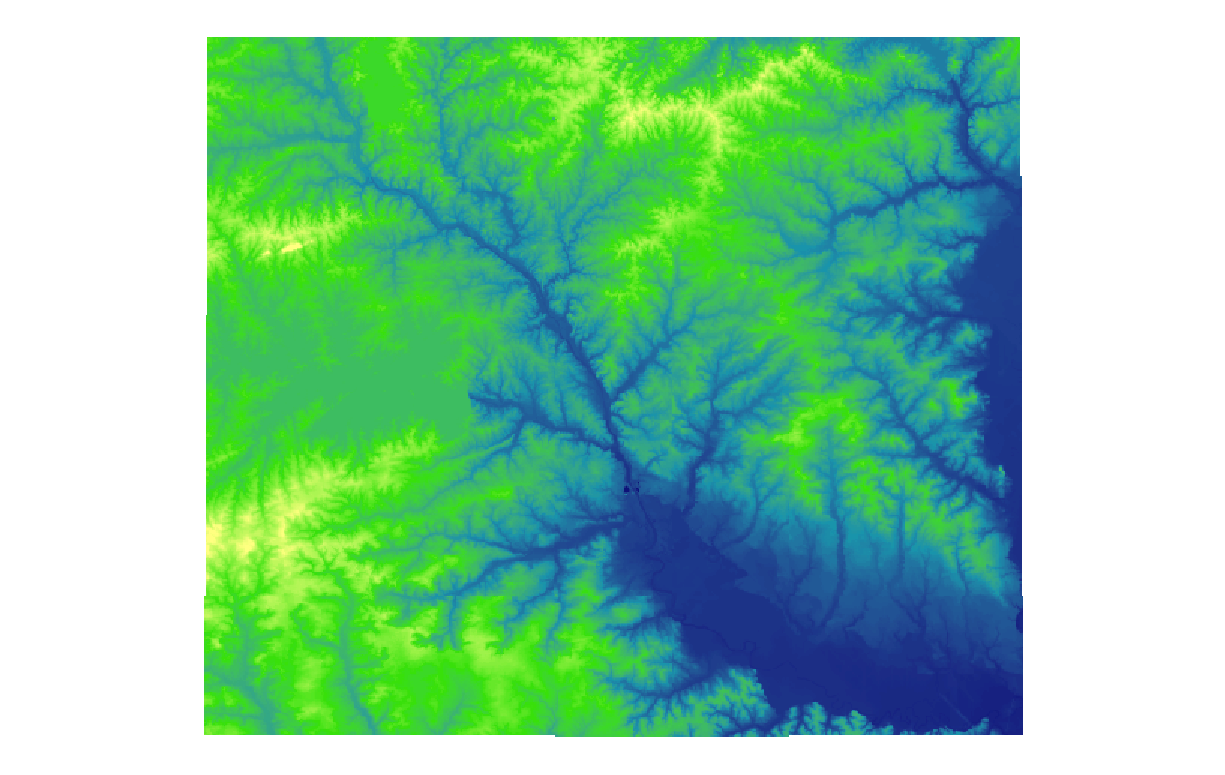
\includegraphics[width=\linewidth]{all.pdf}
\caption{Congaree Confluence Zone - Columbia, SC} \label{fig:ccf}
\end{figure}
There is much interest over the effect of the control of these two
rivers upon the Congaree National Park area that is roughly 25
miles from the confluence of the two rivers.  The Broad has over
two times the streamflow of the Saluda, but the Lake Murray dam is
much closer to the confluence zone and therefore gets much more
attention.   In both rivers, streamflow is more dependent on dam
release than any other factor except for high flows on the Broad
River.

The Saluda is a popular river and is highly utilized by sportsmen
and those looking for a cool place to swim during the hot summers
in Columbia.  The very low temperature (16-18 C) is due to the
draft of the water from the bottom and middle layers of Lake
Murray.  The depth of the draft of the water also has an effect on
dissolved oxygen content of the upper Saluda, but this effect will
not be considered in this paper.

The Broad River is overlooked by many due to its more remote
location and relatively few recreational areas developed for
public use.  It is possible that this lack of attention
contributes to the lack of attention it has received in the
complaints over the management of the Saluda in respect to the
Congaree Swamp and recreation areas downstream of the confluence
zone.  It is clearly apparent from looking at streamflow data that
the Broad River does have considerably more streamflow during all
conditions, whether drought or flood.  For example, during the
summer of 2001, the Saluda consistently ran about 290 CFS (cubic
feet per second) while the Broad ran in the vicinity of 2000 CFS.
The Broad also appears to be just as highly managed as the Saluda,
both being highly tied to power generation.

The effect of both dams on the Congaree National Park is
attenuated by the distance between measuring stations and possibly
the natural smoothing of the flow by obstructions, deepening and
shallowing, and tributaries and runoff from precipitation events.
The Lake Murray dam is closer, so it may have a more direct effect
on the flow of the Congaree as long as the Broad remains
relatively quiet, but the volume of the Broad probably gives it
the upper hand.

What is the relationship between the Saluda and the Broad Rivers
in terms of their combined effect on the Congaree River?  How is
this effect attenuated by the Congaree River's 25 mile reach above
the Congaree Swamp?

The primary method that will be used in determining the
relationship between these rivers will be the multiple input
transfer function model.  In Chapter 2 and Chapter 3 it will be
shown how we will apply transfer function modelling to streamflow
and river stage data.  We will discuss three specific models in
Chapter 4 and analyze some more sophisticated techniques for model
determination in Chapter 5.

\chapter{ARIMA Transfer Function Modelling}
In dynamic systems such as these rivers, it would be ideal to have
continuous information but instead we have hourly measurements.
For the continuous case, we can visualize river segments between
measuring stations as a system of interconnected reservoirs with
the measurements at the the upstream and downstream stations being
the measurement of the level of water in the reservoirs as
described in Box, Jenkins and Reinsel.

With river flows the system becomes a bit more complicated.  The
flow between measurement points is unidirectional in a non-tidal
system.  Also, equilibrium indicates complete absence of water in
the system.  If we consider the flows from both of the input
rivers to be fixed, then the management of the rivers by changing
the amount of water flowing over or through the dam yields a
forcing function-the transfer function. By interpreting how the
changes in the input flows correspond to the output flow we can
determine the transfer function.  From analyzing the transfer
function we can see how the management of the river affects
downstream river conditions.

Unfortunately, the profiles of both of the input rivers change
wildly over time.  This is due to many effects, but mostly to
large precipitation events upstream and the effect of power
production during dry times.  Small time frames are chosen from
the data when the river flows are fairly stable.

Once suitable time frames are selected, a Box-Jenkins transfer
function ARIMA model is fitted to the system.  Then once the input
data has been transformed, ARIMA models are fitted for each input
series. The diagnostics used to determine model accuracy are the
Autocorrelation Function (ACF) and the Partial Autocorrelation
Function (PACF)--both obtained on the residuals of each series. It
is also necessary to check for cross correlation between the input
series.

Once acceptable ARIMA models for the input series have been
fitted, the output series is filtered against both of the input
series. This is done to de-trend the output series based upon what
effect the input series will have on it. At this point the Cross
Correlation Function (CCF) for the system is calculated and
examined.  The delay parameter can be usually judged from the
graph of this function as well as the parameters of the transfer
function. Sometimes the cross-spectrum of the input and output
series can be more useful in determining the delay parameter.

Using the delay, denominator and numerator transfer function
parameters, the transfer function is fitted against the system.
The ACF and PACF of the system residual series is checked and
forecasts are generated. The model autocorrelation of residuals
and cross correlation between input series should not be
significant, and the forecasts should look stable and should be
accurate against hold-out data.

\section{The Box-Jenkins ARIMA Model}
\subsubsection{Autoregressive Processes} A regression model can be
written
\begin{equation}
\tilde{y}=\beta_{1}\tilde{x}_{1}+\beta_{2}\tilde{x}_{2}+\beta_{3}\tilde{x}_{3}+\cdots+\beta_{p}\tilde{x}_{p}+\epsilon
\end{equation}
The time correlated counterpart to the regression model is the
autoregressive model, or AR model.  In the autoregressive model,
the value $z_{t}$ is regressed on its previous values using a time
index.  The general autoregressive model looks like
\begin{equation}
\tilde{z}=\phi_{1}\tilde{z}_{t-1}+\phi_{2}\tilde{z}_{t-2}+\phi_{3}\tilde{z}_{t-3}+\cdots+\phi_{p}\tilde{z}_{t-p}+a_{t}
\end{equation}
representing an $AR(p)$ model.  The autoregressive operator $\phi$
can be described
\begin{equation}\phi(B)=1-\phi_{1}B-\phi_{2}B^{2}-\cdots-\phi_{p}B^{p}\end{equation}
or $\phi(B)\tilde{z}_{t}=a_{t}$ where $B=t-1$ and $B^{p}=t-p$ on
the time index $t$.  This model has $p+2$ unknown parameters which
must be estimated from the data:
$\mu,\phi_{1},\phi_{2},\dots,\phi_{p}$.  The variance
$\sigma_{a}^{2}$ of the white noise process $a_{t}$ is the other
parameter.


\subsubsection{Moving Average Processes}
The difference between the autoregressive and moving average
models is that a autoregressive model constitutes a finite
weighted sum of $p$ previous deviations of the process plus the
error term $a$ while a moving average relates the process to the
error term itself.
\begin{equation}
\tilde{z}=a_{t}-\theta_{1}a_{t-1}-\theta_{2}a_{t-2}-\cdots-\theta_{q}a_{t-q}
\end{equation}
The moving average operator $\theta$ of order \textit{q} is
denoted by
\begin{equation}
\theta(B)=1-\theta_{1}B-\theta_{2}B^2-\cdots-\theta_{q}B^q
\end{equation}
So then the autoregressive operator uses the previous values of
the series, while the moving average operator works on the
previous error terms. A combination of the AR and MA operators is
possible, resulting in an ARMA model which has the form
\begin{equation}
\tilde{z}=\phi_{1}\tilde{z}_{t-1}+\phi_{2}\tilde{z}_{t-2}+\phi_{3}\tilde{z}_{t-3}+\cdots+\phi_{p}\tilde{z}_{t-p}+
a_{t}+a_{t}-\theta_{1}a_{t-1}-\theta_{2}a_{t-2}-\cdots-\theta_{q}a_{t-q}
\end{equation}
The I in the ARIMA model results from differencing, a procedure
that subtracts observed time series values one from another in
some defined scheme.  This operation helps to deal with
nonstationarity and seasonal and unspecified periodicity.
Differencing can be very useful in achieving an appropriate model,
but can make explanation of the model difficult.

\subsection{Transfer Function Models} A \textit{transfer
function} model is a time series model in which one or more input
variables are used to determine the future state of an output
variable.  The transfer function essentially maps the change in
the inputs to the output.

The transfer function transfers the effect of the input variables
using what is called an \textit{impulse response function}.  The
impulse response function waits a certain period of time (delay)
before starting, then applies the input variable in a specific
pattern.

If we consider the continuous case, the first order differential
equation representing a single input \textit{$X$} and a single
output \textit{$Y$} is:
\begin{equation}
(1+T_1 D)Y_1 (t)=g_1 X(t-\tau)
\end{equation}\label{eq:diffeq}
where $\tau$ is the delay, and $g_1$ is the gain (a scaling
factor). $T_1D$ indicates that the rate of change in $Y$ depends
on the difference between $X$ and $Y$.


If higher order models reflect additional dependencies of $Y$ on
$X$:
\begin{equation}
(1+\Xi_1 D + \cdots +\Xi_R D^R)Y(t)=g(1+H_1 D+\cdots+H_S D^S)
X(t-\tau)
\end{equation}
In this equation the $\Xi$ terms result from intermediate
reservoir effects. The $H$ terms represent increasing complexity
in the relationship between the rate of change and the behavior of
$X$.

The continuous model can be represented as a discrete system by
the difference equation:
\begin{equation}
(1+\delta_1 B + \cdots +\delta_r B^r)Y_t=g(\omega_1-\omega_2 B
-\cdots-\omega_ B^s) X_{t-b}
\end{equation}

or

\begin{equation}
\delta(B)Y_t=\omega(B)X_{t-b}
\end{equation}

The standard form of the transfer function with output variable
$Y_{t}$ and input variable $X_{t}$ can be written
\begin{equation}\label{eq:trf}
Y_{t}=\frac{\omega(B)}{\delta(B)}X_{t-b}+N_{t}\\
\end{equation}

 The $\omega$'s are analogous to the autoregressive part of
a time series while the $\delta$'s are analogous to  the moving
average part. The \textit{b}'s represent the general delay in the
impulse response function, or the amount of time before the
impulse response function "activates." This becomes more obvious
if equation (\ref{eq:trf}) is written

\begin{equation}
\delta(B)Y_t=\omega(B)X_{t-b}+N_t
\end{equation}

$N_{t}$ is the noise series of the model and effectively describes
the stochastic part of the dynamic time series model:
\begin{equation}
N_{t}=\frac{\theta(B)}{\varphi(B)}a_{t}
\end{equation}

\subsection{Fitting Transfer Function Models}

To estimate an appropriate transfer function model the input time
series must be analyzed, and appropriate ARIMA models identified.
These models are first used to \textit{prewhiten} the output
series. Prewhitening involves filtering the output series with the
model of the input series; both series are assumed to have no
trend.  This de-trending could be also accomplished by
differencing. Prewhitening removes the direct influence of
autocorrelation in the input series while preserving the important
features of the transfer function model.

The cross correlation function yields a good bit of information
about the delay in the system.  It is not always a good indicator
of the \textit{r} and \textit{s} components, but tentative orders
for the $\omega(B)$ and $\delta(B)$ can be identified. If the
cross correlation function is not helpful in determining delay,
then the cross spectrum of the input with the output series might
help.

Following the prewhitening step, the cross correlation function is
fitted and examined for system wide lags in effect. In other
words, the delay in the first series that affects the second
series is identified.

Once the orders of the input series have been identified, a
tentative ARIMA transfer function model is fit.  This tentative
model may or may not be a good fit, but the results can be used to
identify the delays, and the r and s orders that will yield a good
model fit.

At this point, the error is assumed to be due to an unidentified
process, and an ARIMA model is fitted to the residuals it so that
it can be combined into a systemwide model.  This model, if
accurate enough, can then be used for a variety of purposes.
Forecasting of future output values based on past and current
values of the input series is often the goal.

\subsection{Model Diagnostic Procedures}
In theory, the diagnostic procedures for transfer function models
are rather straightforward.  The residuals should be uncorrelated
with the input series and should look like white noise. They
should also not be cross-correlated with the input time series. If
the residuals have any structure at this point, they should be
modelled into a noise series, such that the remaining residuals
look like white noise.

All this is important, but let us consider the random shock
$a_t=N(0,1)$ in reverse of what is usually done . This is the
building block of our data and is the stochastic part of
everything that follows. From this we assume that there are
patterned inputs, functions that affect the output. These are
applied to the $a_t$ resulting in a patterned behavior based on a
fixed interval of time, a Time Series.

Now, consider the variables that are available in streamflow
modelling:  Precipitation, power generation, the shape of the
stream bed, tributary influence, stream bed absorption,
evaporation and any other unconsidered notion. Chances are that
most of these variables have a very small influence such that the
influence cannot be distinguished statistically from white noise.
In the case of this analysis, we have streamflow data in the form
of flow and stage for four monitoring stations, each with a
different subset of precipitation basins, river bed profile,
average temperatures etc.  The bottom line is that there is
probably a lot of variation in the variable that we are trying to
model, whether it be flow or stage.

But the goal is not to develop a specific model for each of the
variables (which we do not know exactly) but to develop a
predictive model that can shed some light onto the characteristics
of this system of rivers.  For this reason, great care must be
taken when interpreting the diagnostic results. As usual, an
attempt will be made to ensure that the diagnostic statistics are
as reasonable as possible, but I employ a practical method as
well. For each sequence, the forecast is compared against a period
of "hold out" values to determine how well the model holds up for
a short duration. Another indication of model specificity is the
90\% confidence bands that are produced by PROC ARIMA. This is a
visual inspection only at this point, but the more stable the
prediction interval the better.

\chapter{Multiple Input Transfer Function Models for River Data}\label{chp:anal}

\section{The Broad-Saluda-Congaree River System}
The Congaree River is formed by the confluence of the Broad and
Saluda Rivers in the vicinity of downtown Columbia, South
Carolina. The confluence zone is located between the I-126 bridges
and the Jarvis Klapman Bridge, or SC 12, west of Columbia, South
Carolina.

The Broad has the larger flow of the two, usually being three to
five times higher in cubic feet per second (cf/s or cfs). The
Broad, at this point, is managed by the Parr Shoals Dam which is
located roughly 24 miles upstream near Peak, South Carolina and
falls almost 98 vertical feet.

The part of the Saluda River of interest starts at the Lake Murray
Dam, approximately 10 miles from the confluence zone, covering
about 45 vertical feet over that distance.  The streamflow of this
part of the Saluda is a tightly controlled since the Lake Murray
Dam's purpose is power production.

There are four measuring stations of interest to this analysis
displayed in the following table:

\begin{table}[pt]\begin{tabular}{|c|c|c|c|c|} \hline
  % after \\: \hline or \cline{col1-col2} \cline{col3-col4} ...
  \textbf{River} & \textbf{Station Name} & \textbf{Station}& \textbf{ Altitude} & \textbf{Drainage Area}\\
  \hline
  Broad & Alston & 02161000 & 211.91 ft. & 4790 mi$^2$ \\
  Saluda & Below LM Dam & 02168504 & 170 ft. & 2420 mi$^2$ \\
  Saluda & Above Columbia & 02169000 & 149.46 ft. & 2520 mi$^2$ \\
  Congaree & Columbia & 02169500 & 113.02 ft. & 7850 mi$^2$ \\
  Congaree & Congaree Swamp NP & 02169625 & 90.84 ft. & 8290 mi$^2$ \\
  \hline
  \end{tabular}  \caption{Streamflow Monitoring Stations}\label{tab:SMS}
  \end{table}

\subsection{General Analytical Concepts}
It is desired to determine whether or not it is possible to
develop a predictive dynamic forecasting model of the flow (or
stage) of the Congaree River at the Congaree River at Columbia and
the Congaree National Park site.  The twist to this analysis is
that the input series (Saluda and Broad Rivers) are usually quite
correlated. This violates one of the primary assumptions of the
transfer function model, but a good predictive model may still be
possible if careful attention is given to choices of parameters.

Casual observation of the data shows that there are vast
differences in the streamflow of both feeding rivers (Saluda and
Broad).  It is extremely unlikely that an all purpose model is
possible for modelling all situations of streamflow of these two
rivers.

We have identified five different macroscopic views of the flow of
this riverine system for analysis purposes:
\begin{table}[h]
\begin{tabular}{|c|c|} \hline
 \textbf{Streamflow} & \textbf{Definition} \\
  \hline
Flood Conditions & Highly erratic flow where overbank conditions
apply\\
High flow & Large precipitation events or dam discharge on both
rivers\\
Normal Flow & Moderately managed situation on both rivers\\
Low Flow & Highly managed situation on both rivers\\
Drought Conditions & Flow is dependent on dam release only\\
\hline
\end{tabular}\caption{Defined Streamflow Levels}\label{tab:SFCond}
\end{table}

There are a vast number of combinations that would need to be fit
to accommodate every scenario, and the quality of the data is such
that fitting a few well-behaved sequences of data are desired.

\subsection{Dealing With The Data} The data that was used for this
analysis was provided by the United States Geological Survey for
the State of South Carolina.  The data range for the entire input
dataset is January 1, 1995 through October 1, 2002.  This range
was further filtered into three time periods
\begin{table}[h]
\begin{tabular}{|c|c|} \hline
\textbf{Date} & \textbf{Features} \\
\hline
September 5-10, 1996 &
Management of both the Broad and Saluda
Rivers \\
July 21-23, 1995 & Management of the Saluda River while the Broad
River is stable \\
April 28 - May 7, 1999 & Management of the Broad River while the
Saluda River is stable \\
\hline
\end{tabular}\caption{Data Analysis Time Periods}
\end{table}

\subsubsection{Making the Data Analyzable}
The data were received in individual sets organized by streamflow
monitoring station.  Each of these files contained hourly
observations of streamflow, stage, date, hour and minute.  Each of
these files were transformed to contain the following columns:
DATETIME, STREAMFLOW, STAGE, LN(STREAMFLOW), and LN(STAGE).  These
files were then merged by DATETIME, which is a SASDATE datatype.


\subsubsection{Imputation of Missing Values}
Time sequences were chosen to avoid the missing value problem.
Early on, missing values were replaced with the mean for the time
sequence.  This is a rather poor technique for imputing missing
values so series were chosen to avoid this problem
altogether\footnote{PROC EXPAND in SAS is an ideal choice for
imputing missing time series data.}

\subsubsection{Datasets}
The data originated from the US Geological Survey of South
Carolina's streamflow monitoring system.  This system is comprised
of several hundred remote sensors that record the stage of the
river or body of water.


\section{Subsystems}
The analysis of this river system has been divided into two
sections for convenience.  The first section has the Broad and
Saluda Rivers as input series to the Congaree River at Columbia.
The second has Congaree at Columbia as the input and Congaree
Swamp National Park as the output. It makes sense to divide the
system up in this way because of the natural configuration and the
distances involved between measuring stations.

\subsection{Stage 1: Saluda Broad Congaree System}
For the purposes of this analysis, the Saluda River will begin at
the base of Lake Murray Dam.  This is a large impediment to
natural flow and the flow of the river. Lake Murray also has a
great reservoir capacity.  Natural flow rarely occurs on the river
below Lake Murray.

The Broad River is likewise controlled by the Parr Shoals Dam, but
the upstream flow of the Broad is much higher, and the reservoir
capacity of Parr Shoals Reservoir is fairly small.  It is apparent
from the flow diagrams that the Parr Shoals Dam is pretty good at
controlling the flow of the Broad River below the dam until the
river reaches moderate flood conditions.

\section{Delays}
One of the problems with ARIMA transfer function model
determination for streamflow data is that the delay parameter is
likely to change for different streamflow patterns.  It was
hypothesized using empirical knowledge that the amount of delay
from station 1 to station 2 would decrease with increased volume.
This makes physical sense due to the fact that the stream velocity
will increase when the volume increases.



The figures (\ref{fig:brddel}) and (\ref{fig:saldel}) show the
delays of the Broad and Saluda Rivers, against the Congaree at
Columbia. These are not the raw cross correlation functions but a
prewhitened fit taking all inputs into account.  The
crosscorrelation function was calculated on consecutive 7 day
intervals starting on January 1, 1996 and going through the end of
the data.
\begin{figure}[h]
\centering\includegraphics[width=4in]{graphics/BroadDelays.png}
\caption{Comprehensive Delays of Lags vs. Streamflow for Broad
River}\label{fig:brddel}
\end{figure}


\begin{figure}[h]
\centering\includegraphics[width=4in]{graphics/SaludaDelays.png}
\caption{Comprehensive Delays of Lags vs. Streamflow for Saluda
River}\label{fig:saldel}
\end{figure}
This data, like all streamflow data, is rather messy. There is not
much information to be gained from an in depth study of the
results of this analysis, but it can be seen that the bulk of the
results for the Broad River lie between lags 5 and 14. The lag is
negatively correlated with the log of the streamflow in this
vicinity.  For the Broad, the river distance between the Alston
and Columbia stations is roughly 20 miles.  It is unlikely that
the average current velocity would be more than 5 miles per hour
so lags of 0-4 are most likely representative of noise or aliasing
in the data.


Performing the same analysis on the Saluda River yields results
that are similar in nature. The lag again is negatively correlated
with the log of streamflow.  A lag of 1 is unlikely, but lags of 2
through 5 are physically possible.  Lags 8 or larger are also
unlikely and are probably a result of aliasing.  We will see that
lags near 3 build good models.

\section{Description of the Data}
\subsection{Rivers}
The analysis is divided into two parts: a multiple input transfer
function model comprising the Saluda-Broad-Upper Congaree and a
single input transfer function model made up of the Upper
Congaree-Congaree Swamp.

When references are made to the Saluda River, the data was
recorded at the United States Geological Survey Streamflow
Monitoring Station 02168504 which is located just below Lake
Murray Dam.  The Broad River means SC-USGS station 02161000 at
Alston, or Peak, SC. The Upper Congaree, Congaree at Columbia, or
simply Congaree, is station 02169500.  The Congaree Swamp National
Park station is 02169625, and is located near Congaree National
Park.

For the analysis of the multiple input system upstream, streamflow
is used as the variable.  The single input system below Congaree
and Congaree Swamp utilizes the Stage variable since streamflow
was unavailable for most of the dates in the dataset.

Streamflow is measured in cubic feet of water per second passing a
specified point, and is often derived from the stage data
mathematically.

Stage is the familiar height of the river above or below some
datum.  Stage is measured in feet for all of the gauges used in
this report.

\subsection{Methods of Analysis}
All of the following analysis was performed using SAS/ETS
software, primarily PROC ARIMA.  Target time periods were selected
by visually inspecting monthly profile graphs of the data from all
of the stations.  The time periods were further refined using
trial and error to sections of data that could be modelled with
reasonable accuracy.  As mentioned in the section on data
imputation, time periods were also selected where missing values
did not occur.

It was decided early on not to difference the data.  Since river
related data is notoriously hard to model, this made finding
representative timeframes fairly difficult.

\subsubsection{Prewhitening of Inputs}
For all analyzed time periods, a visual inspection of the input
ACF, PACF, and CCF graphs was done in an attempt to identify model
parameters. Since differencing was not a primary focus, this did
not lead to a very good estimation of the p and q components of
the model. Both the Saluda and Broad Rivers were subjected to a
trial and error approach using a SAS/AF application
(\ref{fig:SASAF}) that was developed to expedite the trial and
error process.  The idea behind the trial and error process is to
pick AR and MA components such that the autocorrelation of
residuals and the cross correlation between the inputs and the
white noise of the residuals is negligable.

 The primary method of determining input
\textit{p} and \textit{q} parameters was using the output from the
SCAN option of PROC ARIMA's IDENTIFY option. SCAN (Smallest
Canonical correlation) analyzes the eigenvalues of the correlation
matrix of an ARMA process and returns a matrix of possible
autoregressive and moving average parameters. This criterion
usually produced the best models, and saved time during the trial
and error step.

\subsubsection{Delay
Parameters} The delay between each input and the output was also
investigated at this time.  This was done by looking at the
largest absolute value of the cross correlation function over a
lag spread of -24 to 24. There is no physical reason why the lag
should ever exceed these parameters.  This was a tricky part of
the analysis since the delays were often aliased, or correlated
with larger or smaller multiples of themselves.  It is also
possible that interference patterns caused the CCF analysis to be
non-specific. A good bit of common sense went into picking the
most appropriate lag for each prewhitening input.

\chapter{Data Analysis}
Targets of opportunity for analysis were selected by looking at
monthly flow and stage profiles at the four selected monitoring
stations.  Acceptable targets were time periods with a low
incidence of missing data, visible stationarity, and situations
where it was obvious that river management was occurring.  Even
with hourly data for seven years, this was an easy exercise.

\section{September 5-10, 1996 - High Management On Both Rivers}
\subsection{Logged Streamflow Modelling}
\begin{figure}\label{fig:sepfl510}
\centering\includegraphics[width=4in]{graphics/05sep96FlowPRF.png}
\centering\caption{Flow Profile Plot for September 5-10, 1996}
\end{figure}

A quick look at the logged streamflow profile for this period
shows a well-behaved system.  The five days of hourly data should
give enough data to generate a good model.

The ACF of the Saluda River (Figure \ref{fig:sepflowacf}) data
shows that the series may benefit from differencing the data
before analysis. The PACF of the Saluda data (Figure
\ref{fig:sepflowacf})
 shows that this river might be modelled using an AR(2) component.

The ACF of the Broad River data shows that the series could also
benefit from differencing the data before analysis. The PACF of
this data shows that this river might be modelled using an AR(2)
or an AR(3) component.
\begin{figure}[h]
\centering\includegraphics[width=4in]{prodgraph/05sepinputdiag.png}
\centering\caption{Input Series ACF and PACF Plots for September
5-10, 1996}\label{fig:sepflowacf}
\end{figure}

\begin{figure}[h]
\centering\includegraphics[width=4in]{graphics/05sep96FlowCCF.png}
\centering\caption{Streamflow Cross-Correlation Plot for September
5-10, 1996}\label{fig:sepccf}
\end{figure}

The cross-correlation function for this period (Figure
\ref{fig:sepccf}) shows that the Saluda delay is about three
hours.  This holds well with other observations and historical
averages.  The delay for the Broad River looks to be 10 hours.
Again, this holds well with observational evidence.

There is a stronger negative correlation for the Broad River at 11
hours and a very strong positive correlation at 0 hours.  The 0
hour value probably is indicative of the correlation between the
input series and is obviously false based on the physical nature
of water and the distances between these two monitoring stations.
The 11 hour correlation is interesting. Note that in most of the
examples shown, the maximum absolute correlation will occur among
a range of nearby lag values.  Here it is 8, 10 and 11.  The
method for determining the best delay to use for the model was
based upon the model fit diagnostics.


A quick look at the ACF and PACF(Figure \ref{fig:sepflowacf})
graphs for the input variables and the pre-whitened, system-wide
data shows some valuable information for model building.  All of
the ACF's show a slow tail-off, usually indicating the need for
differencing of the data.  The data is not differenced in this
analysis because it is desired to see if reasonably accurate
models can be built without differencing.  The one-step-ahead
forecasts are of particular interest.  Obviously, some of the
assumptions of the ARIMA model will be violated.  This does not
mean that a fairly accurate predictive model cannot be created.


\begin{figure}[h]
\centering\includegraphics[width=4in]{graphics/05sep96FlowFCST.png}
\centering\caption{Streamflow Forecast Plot for September 5-10,
1996}
\end{figure}

The forecast for this period is fairly stable.  Often with
transfer function models the forecast standard errors diverge
quickly from the forecast itself.  In this case it is obvious that
the actual flow changed from the pattern that was used to create
the model.  The one step ahead forecasts for the series follow the
data very well.

\begin{table}[h]
\centering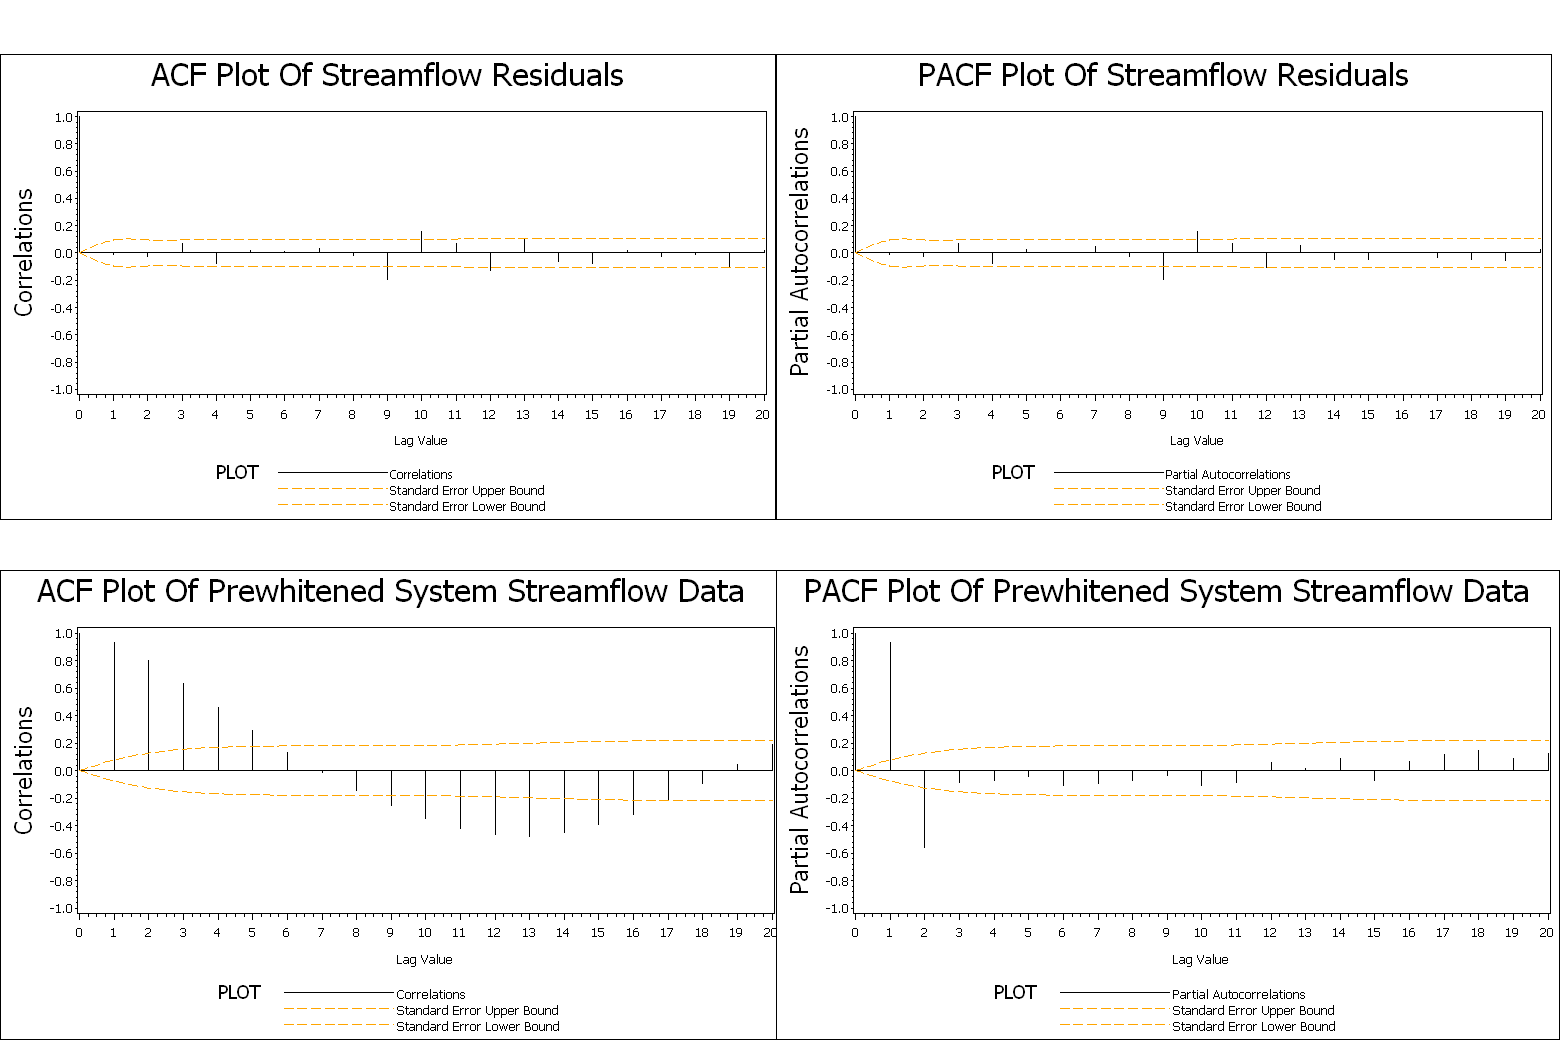
\includegraphics[width=4in]{prodgraph/05sepresid.png}
\centering\caption{System  Diagnostics for September 5-10,
1996}\label{fig:resacf12}
\end{table}

\begin{table}[h]
\begin{centering}
\begin{tabular}{|c|c|c|c|}
\hline
\textbf{River}  & \textbf{AR} & \textbf{MA} & \textbf{Delay} \\
\hline Broad & 2 & 0 & 10 \\
Saluda & 2 & 1 & 3 \\
Congaree (model) & 2 & 1 & - \\
\hline
\end{tabular}\caption{Streamflow Model Parameters for September 5-10 1996}
\end{centering}
\end{table}

The transfer function model, modelled as an ARMA(2,1) follows:


\begin{equation}
\begin{split}
\label{eq:5sepmodel}
CAC_t=4.53&+\frac{0.11246+0.01779 B^1}{1-0.55418 B^1}SAL_{t-3}\\
&+\frac{0.09085-0.0852 B^1}{1-0.97935 B^1}BRD_{t-10}\\
&+\frac{1+0.01546 B^1}{1-1.29681 B^1 + 0.49662 B^2}\eta_t\\
\end{split}
\end{equation}

\subsubsection{Diagnostics}
Using the Basic fit diagnostics involves making sure that the
residuals are not autocorrelated, nor are cross correlated with
the input data. It is clear from \ref{tab:sepModDiag} that this
model passes the residual checks.  The fact that the $\chi^2$ test
p-values are large for the cross-correlation of the residuals with
the input series indicates that the transfer function model is
correctly specified. The $\chi^2$ test p-values for the
autocorrelation of the residuals being large indicates that the
input ARIMA model for the output series is correctly specified.

Finally, the residual series is again considered to determine if
any structure still exists.  If so, then it may be possible to
further refine the model.  The $chi^2$ test p-values (Figure
\ref{fig:resacf12}) are quite large for the test that the residual
series has structure remaining. It is safe to say that no
appreciable structure remains in the residuals and the model is
adequately specified.


\subsection{Stage Modelling}%
\begin{figure}[h]
\centering\includegraphics[width=4in]{graphics/05sep96StagePRF.png}
\centering\caption{Stage Profile Plot for September 5-10, 1996}
\end{figure}
The profile for this period looks like a good candidate for
dynamic transfer function modelling.  There does seem to be some
linear trend, and the ACF (\ref{fig:sepstagediag}) of the input
shows the classic pattern of slow alternating decay that suggests
differencing the data. Again, it was chosen not to difference the
data to determine if model building is possible under this
limitation.  The PACF for this period hints at the input Congaree
at Columbia being satisfactorily specified using an AR(2)
component.

Using a trial and error approach via the SAS/AF modelling
application developed for this purpose (\ref{fig:SASAF}) a
ARMA(2,1) model was chosen for the input variable.  This model is
used to pre-whiten both the input and output series and then these
pre-whitened series are analyzed to determine the model
parameters.  The pre-whitening filter is:

\begin{equation}\label{eq:congStagPrewhitenFilter}
CAC_t=1-1.52924B+0.61964 B^2
\end{equation}

The pre-whitened model ACF (Figure \ref{fig:sepstagediag}) again
shows the possible need for differencing. The PACF is a little
more useful, showing a possible AR(3) component to the model.

The cross-correlation function of the Congaree at Columbia vs.
Congaree Swamp \ref{fig:sepstageccf} shows a difficult situation
where there is no real indication of the delay in the system. It
may be explained by looking at the profile plot itself.  The
offset of the series are almost completely in interference with
each other--making the cross-correlation function misleading for
this series. The greatest absolute values for the CCF as-is yields
a delay of one or two hours, both of which are physically
improbable.  The span of lags 6 to 12, corresponding with 6 to 12
hours, are much more feasible, and the CCF does hint that there
may be something there. In the end, trial and error was used to
determine the delay within this range that yielded the best
diagnostic values.
\begin{figure}[h]
\centering\includegraphics[width=4in]{graphics/05sep96StageCCF.png}
\centering\caption{Stage Cross-Correlation Plot for September
5-10, 1996}\label{fig:sepstageccf}
\end{figure}
A delay of 9 hours and an ARMA(3,2) appears to be the best fit for
the model using the trial and error approach through the SAS/AF
application.

\begin{figure}[h]
\centering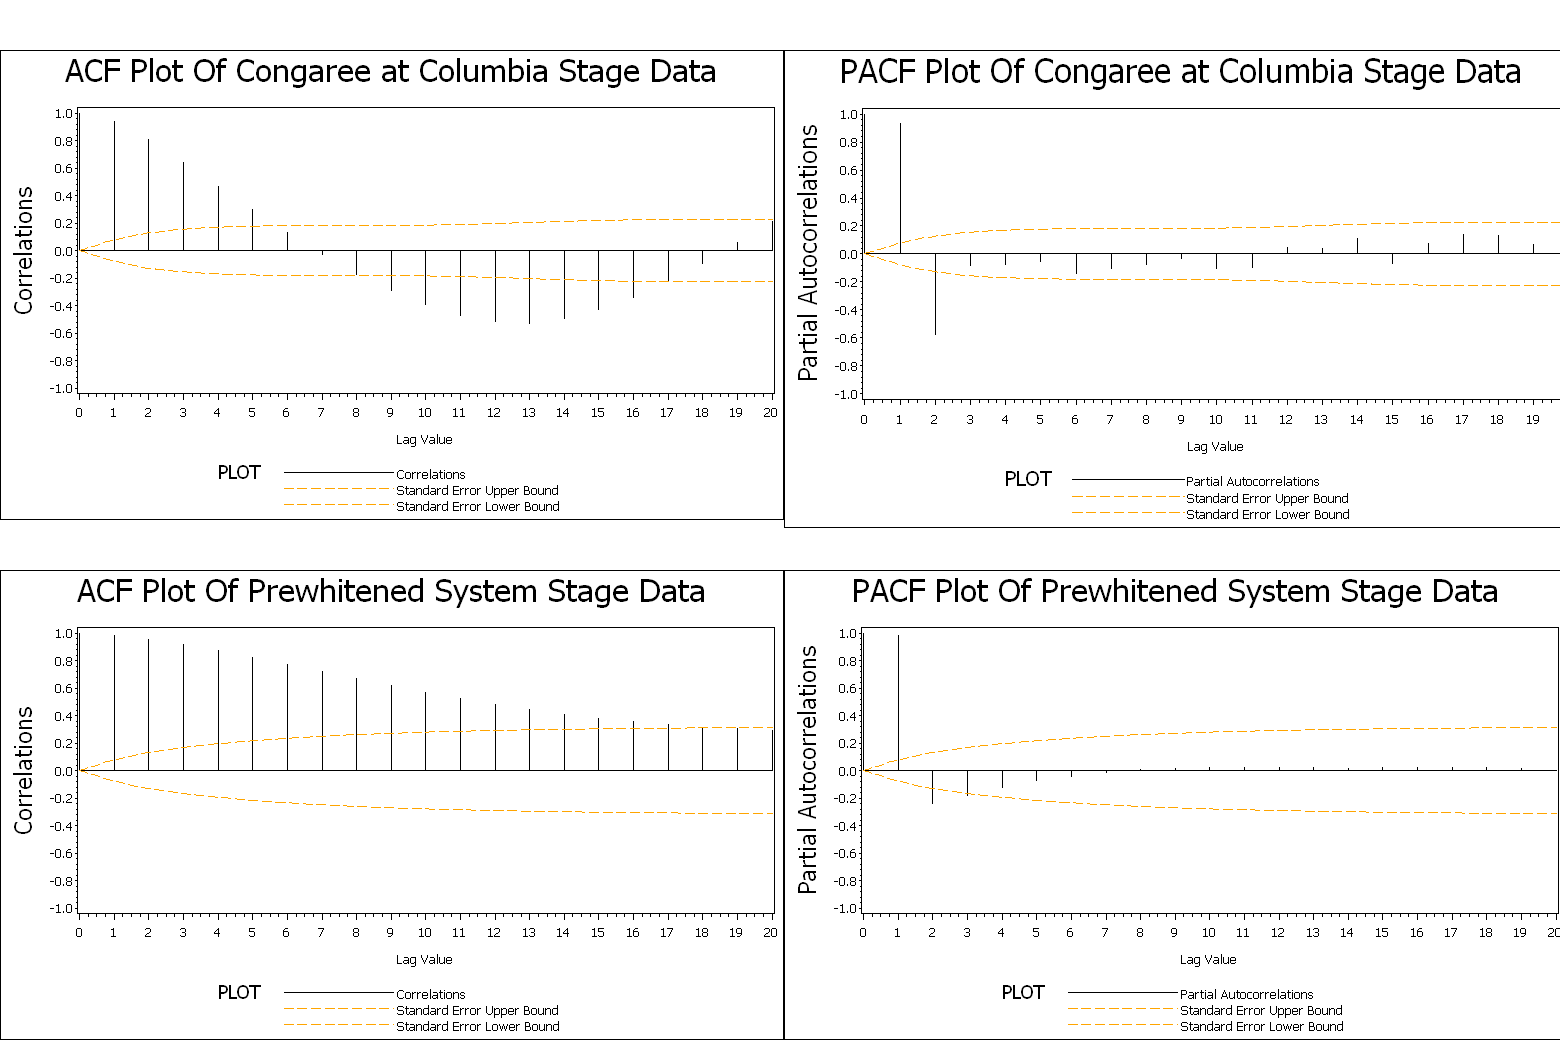
\includegraphics[width=4in]{prodgraph/05sepstagediag.png}
\centering\caption{System Stage ACF and PACF for September 5-10,
1996}\label{fig:sepstagediag}
\end{figure}

Even with the unknown factors, and the difficulty in deciding upon
a delay, the forecast was very good.  In the forecast plot, the
vertical line represents the last data point used in the
calculation of the forecast. The 95\% confidence limits may not be
very useful since they grow to such a large span so fast, but the
actual forecast holds very true to the hold-out data.  The
forecast successfully predicts the trend for three days and very
accurately predicts the actual stage for an entire day.
\begin{figure}[h]
\centering\includegraphics[width=4in]{graphics/05sep96StageFCST.png}
\centering\caption{Stage Forecast Plot for September 5-10, 1996}
\end{figure}


\begin{table}[h]
\begin{centering}
\begin{tabular}{|c|c|c|c|}
\hline \textbf{River} & \textbf{AR} & \textbf{MA} & \textbf{Delay} \\
\hline Congaree at Columbia & 2 & 1 & 9 \\
Congaree at Congaree Swamp (model) & 3 & 2 & - \\
\hline
\end{tabular}\caption{Stage Model Parameters for September 5-10, 1995}
\end{centering}
\end{table}


The stage model estimated to be an ARMA(3,2) for 5-10 September
becomes:

\begin{equation}
\begin{split}
\label{eq:5sepstagemodel}
CSNM_t=10.951&+\frac{0.00143+0.00329B}{1+0.98073B}CAC_{t-9}\\
&+\frac{1-0.1747B+0.48465B^2}{1-2.70765B+2.49887B^2-0.78999B^3}\eta_t\\
\end{split}
\end{equation}

The diagnostics for this model show some of the problems that are
associated with the cross-correlation function problem.  The
autocorrelation of the residuals (Figure
\ref{fig:sepstagemdldiag}) shows a marginal problem out to lag 6,
but no problem whatsoever thereafter.  Furthermore, there is no
reason to assume that the residual series is anything more than
white noise (Figure \ref{fig:sepstagewht}).


Again, the system $\chi^2$ test p-values are large enough for both
the cross correlation with the input series and autocorrelation of
the residuals that we can be comfortable with the model and
transfer function specifications.

The test for white noise of the residual series is likewise
affirmative in that the $\chi^2$ test p-values are large.  This
again indicates that the residual series does not have any
autocorrelation structure and appears like white noise.



\clearpage
\section{July 21-23, 1995 - High Management on Saluda, Constant Flow on the Broad River}
\subsection{Logged Streamflow Modelling}
\begin{figure}[h]
\centering\includegraphics[width=4in]{graphics/21Jul95FlowPRF.png}
\centering\caption{Flow Profile for July 21-23, 1995}
\end{figure}
The time period taken for study is July 21-23, 1995.  This period
was selected because the Saluda River was under heavy management
as evidenced by the regular periodicity in stream flow. This
periodicity relates to the regular afternoon water release by the
Lake Murray Dam.  It is assumed with a very high level of
confidence that this is directly related to increased power need
in the mid-afternoon. The Saluda was also flowing at roughly a
2800 cubic feet per second streamflow average representing a
moderately high flow pattern. The monitoring station for this data
is located less than one mile below the Lake Murray Dam, so will
not suffer much from attenuation effects of tributaries and
rainfall.  Accurate precipitation records for the local drainage
area were not available so this is not considered.

During the same time period, the Broad River streamflow remains at
a fairly constant 3000 cubic feet per second. This combination
makes this time period a good one for studying the effect of the
Saluda River when the Broad River remains constant. In other
words, attenuation effects can be studied without interference of
the Broad River.
\begin{figure}[h]
\centering\includegraphics[width=4in]{prodgraph/23Julinput.png}
\centering\caption{Saluda and Broad River Streamflow ACF/PACF July
21-23, 1995}\label{fig:julfsalapcf}
\end{figure}

\begin{figure}[h]
\centering\includegraphics[width=4in]{graphics/21Jul95FlowCCF.png}
\centering\caption{Flow Cross Correlation Plot for July 21-23,
1995}
\end{figure}
The pre-whitened cross correlation function shows strong evidence
for lags of three and seven hours for the Saluda and Broad River
respectively.

In this time period, a delay of four hours for the Saluda River
and seven hours for the Broad is consistent with most
observations.  It is interesting to note that good fitting models
can be generated using multiples, or near multiples of this value.
Notably, using a delay of four for the Broad River extent yields a
model that would pass the rudimentary criteria that are used here
for model selection. Furthermore, the CCF for the Broad River
shows strongly negative peaks at -7, 4 and 16 lags.

Forecasts for this model are typical for transfer functions:

\begin{figure}[h]
\centering\includegraphics[width=4in]{graphics/21Jul95FlowFCST.png}
\centering\caption{Flow Forecast Plot for July 21-23, 1995}
\end{figure}


\begin{figure}[h]
\centering\includegraphics[width=4in]{prodgraph/23Juldiag.png}
\centering\caption{System Streamflow Diagnostics July 21-23,
1995}\label{fig:julfsysapcf}
\end{figure}

The forecast for this time period looks like transfer function
model forecasts usually do.  The actual values are plotted along
with the predicted values and the $90\%$ confidence intervals for
the ARIMA transfer function model.  The forecast remains fairly
accurate for an entire 24 hour period after the last data point,
even though the series seems to be deviating from the pattern used
to forecast it.

\begin{table}[h]
\begin{centering}\begin{tabular}{|c|c|c|c|}
\hline \textbf{River} & \textbf{AR} & \textbf{MA} & \textbf{Delay} \\
\hline Broad & 0 & 2 & 7 \\
Saluda & 1 & 1 & 3 \\
Congaree (model) & 1 & 1 & - \\
\hline
\end{tabular}\caption{Streamflow Model Parameters for July 21-23, 1995}
\end{centering}\end{table}


The estimated model is then:

\begin{equation}
\begin{split}
\label{eq:21julflowmodel} CAC_t=6.88163&+\frac{0.19344+0.09706
B}{1-0.20714B}SAL_{t-3}\\
&+\frac{-0.0328-0.11652B}{1+0.19723B}BRD_{t-7}\\
&+\frac{1+0.33188B}{1-0.33745B}\eta_t\\
\end{split}
\end{equation}

The model diagnostics (shown in Appendix A Figure
\ref{tab:JulModDiag}) within PROC ARIMA show that the probability
of the residual series not being white noise is very low.  We can
say with confidence that the residual series does not maintain
characteristics of the model itself, and is fairly random.  This
may not be the best fitting model as residual diagnostics go, but
it is well defined and very appropriate for the needs of this
analysis.

\clearpage
\subsection{Stage Modelling}

\begin{figure}[h]
\centering\includegraphics[width=4in]{graphics/21Jul95StagePRF.png}
\centering\caption{Stage Profile Plot for July 21-23, 1995}
\end{figure}

The stage values during this period were analyzed since reliable
flow values were not available.  The profile plot shows a good
deal of attenuation between the Columbia and Congaree Swamp
monitoring stations.  It is also possible to discern the delay
between these two stations.

\begin{figure}[h]
\centering\includegraphics[width=4in]{graphics/21Jul95StageCongACF.png}
\centering\caption{Congaree River at Columbia Stage ACF/PACF July
21-23, 1995}\label{fig:julsconapcf}
\end{figure}


The CCF shows a common problem that was encountered during this
analysis; the greatest correlation is negative and at $b=0$. A
quick look at the profile plot may show why this is occurring. On
the profile plot, the maxima for the Congaree at Columbia occur
very near the minima for Congaree Swamp.  This corresponds with a
strong negative correlation at zero, and can account for the
fairly strong positive correlations at -1 and 1. There is no way
that any perturbation of flow can travel the 25 miles between
these two stations within an hour or so.  In this case it is
necessary to use some common sense.  If we look at the positive
lag values, a maximum occurs at 8.  If the delay was 8 hours as
this peak hints, this would correspond with a streamflow rate of
around 3 miles per hour.  This not only makes sense, but is also a
good estimate for the river at this point.

\begin{figure}[h]
\centering\includegraphics[width=4in]{graphics/21Jul95StageCCF.png}
\centering\caption{Stage Cross-Correlation Plot for July 21-23,
1995}\label{fig:jul21stageccf}
\end{figure}

There is also a strong negative correlation that occurs around the
-11 lag.  This is very interesting, but is also almost certainly
due to aliasing in the data.  This lag was also ignored based on
empirical knowledge, and for the purposes of this analysis.
 \clearpage

\begin{figure}[h]
\centering\includegraphics[width=4in]{graphics/21Jul95StageFCST.png}
\centering\caption{Stage Forecast Plot for July 21-23, 1995}
\end{figure}

As can be seen from the forecast plot, a precise model was
created. The forecast deviated strongly from the actual values,
but this appears to be a change in the profile itself.

\begin{table}[h]
\begin{centering}\begin{tabular}{|c|c|c|c|}
\hline \textbf{River} & \textbf{AR} & \textbf{MA} & \textbf{Delay} \\
\hline Congaree at Columbia & 2 & 0 & 8 \\
Congaree at Congaree Swamp (model) & 2 & 0 & - \\
\hline
\end{tabular}\caption{Stage Model Parameters for July 21-23, 1995}
\end{centering}\end{table}


\begin{equation}\begin{split}
\label{eq:21jul3stagemodel}
CNSM_t=6.012219&+\frac{0.02055+0.000006B
}{1-0.81546B}CAC_{t-8}\\
&+\frac{1}{1-1.81268B+ 0.97588B^2}\eta_t
\end{split}
\end{equation}

One of the difficulties in modelling this type of data is knowing
when the profile changes.  In the case of managed rivers, the
profile changes are related to both manmade (power generation
requirements) and natural (precipitation or lack thereof) sources.
Both of these sources are very difficult to account for.  For
example, power generation can be directly proportional to regional
temperature, but can also be related to lack of power in other
parts of the country.  Precipitation can be related to local
precipitation or precipitation upstream.  Sometimes dams release
water due to flooding instead of primarily power generation.

\begin{figure}[h]
\centering\includegraphics[width=4in]{graphics/21Jul95StagesysACF.png}
\centering\caption{System Stage Diagnostics for July 21-23,
1995}\label{fig:julssysapcf}
\end{figure}


\clearpage

\section{April 28 - May 5 1999 - High Management Constant Flow on the Saluda
River}
\subsection{Logged Streamflow Modelling}
\begin{figure}[h]
\centering\includegraphics[width=4in]{graphics/28APR99FlowPRF.png}
\centering\caption{Flow Profile Plot for April 28 - May 5, 1999}
\end{figure}
This profile looks quite different from the others in that the
Saluda input is quite monotone and flat.  There is a good bit of
variation in both the Broad River and the Congaree River at
Columbia flow profiles.  There is a large dip in the flow of the
Congaree at Columbia around May 6.

\begin{figure}[h]
\centering\includegraphics[width=4in]{graphics/28Apr99FlowsysACF.png}
\centering\caption{Pre-whitened System Streamflow ACF/PACF April
28-May 5, 1999}
\end{figure}

The CCF for this time sequence is again problematic. In fact, the
aliasing is so bad that a decision on delays was made using
knowledge rather than the data.  The Broad River station shows a
strong positive correlation at 6 hours.  This is almost half of
the delay parameter that was seen in previous models for the Broad
River.  It is very possible that the stream velocity could double
due to the increased flow during this period.

\begin{figure}[h]
\centering\includegraphics[width=4in]{graphics/28APR99FlowCCF.png}
\centering\caption{Streamflow Cross-Correlation Plot for April 28
- May 5, 1999}
\end{figure}

The Saluda, since it did not change much over the period, produced
an unusual CCF . This pattern may well be due to the single large
value at the start of the series. For this analysis the standard 3
hour delay is used even though the cross correlation function does
not necessarily specify this.

The ACF and PACF for this period seem to indicate an AR(2) model
for both the Saluda and Broad inputs.  After applying trial and
error to the analysis the following parameters were determined to
yield the best model for this time period:

\begin{table}[h]
\begin{centering}\begin{tabular}{|c|c|c|c|}
\hline \textbf{River} & \textbf{AR} & \textbf{MA} & \textbf{Delay} \\
\hline Broad & 4 & 2 & 6 \\
Saluda & 1 & 1 & 3 \\
Congaree (model) & 5 & 2 & -  \\
\hline
\end{tabular}\caption{Streamflow Model Parameters for April 28-May 5,
1999}
\end{centering}\end{table}

 The model is:

\begin{equation}\begin{split}
\label{eq:28aprflowmodel}
CAC_t=-7.86145&+\frac{0.3354+1.2452B}{1-0.27738B}SAL_{t-3}\\
&+\frac{0.11023+0.11878B}{1+0.18196B-0.73073B^2}BRD_{t-6}\\
&+\frac{1+0.86116B+0.9998B^2}{1-0.40928B+0.05219B^2-0.78709B^3+
0.2729B^4+0.12169B^5}\eta_t\\
\end{split}
\end{equation}

\begin{figure}[h]
\centering\includegraphics[width=4in]{graphics/28APR99FlowFCST.png}
\centering\caption{Streamflow Forecast Plot for April 28 - May 5,
1999}
\end{figure}
The forecast is relatively stable for the first part of the
forecasting period.

\begin{figure}[h]
\centering\includegraphics[width=4in]{graphics/28Apr99FlowResACF.png}
\centering\caption{System Streamflow Diagnostics April 28-May 5,
1999}
\end{figure}

\subsection{Stage Modelling}

\begin{figure}[h]
\centering\includegraphics[width=4in]{graphics/28APR99StagePRF.png}
\centering\caption{Stage Profile Plot for April 28 - May 5, 1999}
\end{figure}

The profile plot for this section shows the regular periodicity
expected of this stretch of the Congaree River and it seems to
attenuate the increase in streamflow seen in the streamflow
profile.


\begin{figure}[h]
\centering\includegraphics[width=4in]{graphics/28APR99StageColAcf.png}
\centering\caption{Stage ACF April 28 - May 5, 1999}
\end{figure}


The CCF for this period is again not particularly helpful. A value
of 7 for the delay was used. This value was arrived upon by
\begin{figure}[h]
\centering\includegraphics[width=4in]{graphics/28APR99StageCCF.png}
\centering\caption{Stage Cross-Correlation Plot for April 28 - May
5, 1999}
\end{figure}
starting with the knowledge that delays in the range of 6-9 have
been used in successful models on this stretch of river.  The
actual value of 7 was arrived at through trial and error.

\begin{table}[h]
\begin{centering}\begin{tabular}{|c|c|c|c|}
\hline \textbf{River} & \textbf{AR} & \textbf{MA} & \textbf{Delay} \\
\hline Congaree at Columbia & 3 & 3 & 7 \\
Congaree at Congaree Swamp (model) & 3 & 2 & - \\
\hline
\end{tabular}\caption{Stage Model Parameters for April 28-May 5,
1999}
\end{centering}\end{table}

The estimated model for stage is:

\begin{equation}\begin{split}
\label{eq:28aprstagemodel} CSNM_t=6.593664&+\frac{ -0.0002 +
0.00562 B**(1) }{1 + 0.89108 B**(1) }CAC_{t-7}\\
&+\frac{1-0.19199B+0.46371B^2}{1-2.67269B+2.40008B^2-0.72665
B^3}\eta_t\\
\end{split}
\end{equation}

The forecasts for the stage are fairly good.  The deviation
between the one step ahead forecasts and the actual values are
fairly small and the long term forecast sticks very close to the
hold out data.


\begin{figure}[h]
\centering\includegraphics[width=4in]{graphics/28APR99StageFCST.png}
\centering\caption{Stage Forecast Plot for April 28 - May 5, 1999}
\end{figure}

\begin{figure}[h]
\centering\includegraphics[width=4in]{graphics/28APR99StageRESACF.png}
\centering\caption{Stage Diagnostics for April 28 - May 5, 1999}
\end{figure}

\clearpage
\section{Delay Determination Using Spectral Analysis}
Although the cross correlation function was useful in determining
the delay between the change in an input and the output, there was
often a discrepancy in what the CCF suggested and what was logical
and what yields a good model.

The cross correlation function for the July 21-23 stage analysis
between the Congaree at Columbia and Congaree at Congaree Swamp
National Park (\ref{fig:jul21stageccf}) is difficult to interpret.
If we calculate the cross-spectra (\ref{fig:21julspect}) of the
river stage without transformation more information is possible.

\begin{figure}[h]\centering
\includegraphics[width=4in]{graphics/21JulStageSpectra.png}
\caption{Spectrum Example 1}\label{fig:21julspect}
\end{figure}
It is clear that there does appear to be a maximum around 11
hours, which is consistent with what is expected.  Using a delay
of 11 hours yielded a reasonably good model fit as well.

The cross-spectra plot does not always provide a good indicator of
the delay parameter however.
\begin{figure}[h]\centering
\includegraphics[width=4in]{graphics/05SepSalflow_Spec1.png}
\caption{Spectrum Example 2}\label{fig:05sepsalspect1}
\end{figure}

Sometimes aliasing, or the superimposition of smaller periods, can
lead to misleading results as in figure \ref{fig:05sepsalspect1}.
Here the maximum occurs around 23 hours.  This length of time
indicates daily patterns, so in this case it might be necessary to
investigate some of the smaller components of this peak to study
delay. In figure \ref{fig:05sepsalspect2} the spectrum is zoomed
in to periods less than 4.  The common pattern of a maximum in the
vicinity of 3 or 4 arises.  It turns out that a delay of 3 yielded
a good model fit.

In this case, the cross correlation plot showed a peak at 3 hours
for the Saluda River (Figure \ref{fig:sepccf}).


\begin{figure}[h]\centering
\includegraphics[width=4in]{graphics/05SepSalflow_Spec2.png}\caption{Spectrum Example 3}
\label{fig:05sepsalspect2}
\end{figure}

Using both the cross correlation function and the cross spectrum
can lead to the delay parameter, but trial and error might still
be necessary to develop a good model.

\clearpage\
\chapter{Conclusions} It is possible to develop decent predictive
models for multiple input ARIMA models for streamflow data.  There
will be no "silver bullet" for such models although it may be
possible to categorize flow periods into a finite set of patterns
which may then be modelled.  It may even be possible to construct
a piecewise ARIMA model for putting these together in a meaningful
way.

Using the multiple input transfer function method we were able to
discover details about the delays between the monitoring stations,
and discovered how the delay is not necessarily constant but
changes with flow.  This will be a serious complication to any
attempt to develop a comprehensive model.



Good predictive models were attainable without differencing. These
usually corresponded to time sequences of three to five days and
contained data that varied in complexity. Both the one step ahead
and the long term forecasts can be fairly accurate when river
management is consistent from day to day.

\bibliographystyle{plain}
\bibliography{uscthesis}
%%%%%%%%%%%%%%%%%%%%%%%%%%%%%%%%%%%%%%%%%%%%%%%%%%%%%%%%%%%%%%%%%%%%%%%%%%%%%%%%%%%%%%%%%%%%%%%%%
%%%%%%%%%%%%%%%%%%%%%%%%%%%%%%%%%%%%%%%%%%%%%%%%%%%%%%%%%%%%%%%%%%%%%%%%%%%%%%%%%%%%%%%%%%%%%%%%%



%Start your appendices, optional.
\appendix
\chapter{Model Diagnostic Results}

\begin{table} \scriptsize
\begin{centering}
\begin{verbatim}

                      ARIMA Model Identification, Estimation, and Forecast
                    Thursday, 5 September 1996 - Tuesday, 10 September 1996

                                      The ARIMA Procedure

                 Crosscorrelation Check of Residuals with Input logsaluda_flow

   To        Chi-             Pr >
  Lag      Square     DF     ChiSq    --------------------Crosscorrelations-------------------

    5        5.14      4    0.2734    -0.028    -0.048    -0.082    -0.143     0.133     0.010
   11        9.25     10    0.5088    -0.107     0.078    -0.101     0.086     0.016    -0.055
   17        9.96     16    0.8688    -0.033     0.036     0.002     0.013    -0.021     0.060
   23       13.25     22    0.9259     0.002    -0.028     0.034    -0.038     0.146     0.078

                 Crosscorrelation Check of Residuals with Input logbroad_flow

   To        Chi-             Pr >
  Lag      Square     DF     ChiSq    --------------------Crosscorrelations-------------------

    5        3.49      4    0.4787     0.066    -0.127     0.082    -0.074     0.047     0.004
   11        9.04     10    0.5284    -0.083    -0.072    -0.040     0.125     0.145    -0.070
   17        9.96     16    0.8687     0.073     0.042    -0.027    -0.010     0.035    -0.003
   23       13.98     22    0.9024    -0.076    -0.133    -0.123    -0.018     0.036    -0.007


                              Autocorrelation Check of Residuals

   To        Chi-             Pr >
  Lag      Square     DF     ChiSq    --------------------Autocorrelations--------------------

    6        1.28      3    0.7334    -0.001    -0.023     0.075    -0.064     0.028     0.007
   12       10.69      9    0.2974     0.028    -0.006    -0.183     0.142     0.073    -0.128
   18       13.53     15    0.5618     0.098    -0.059    -0.085     0.013    -0.040     0.001
   24       17.31     21    0.6919    -0.093     0.014    -0.013    -0.078     0.074    -0.081

\end{verbatim}
\end{centering}
\normalsize\caption{Model Diagnostics for 5-10 September 1996
Streamflow }\label{tab:sepModDiag}
\end{table}
\begin{table} \scriptsize
\begin{centering}
\begin{verbatim}
                            Streamflow Diagnostics for Residual Series

                    Thursday, 5 September 1996 - Tuesday, 10 September 1996

                                      The ARIMA Procedure

                              Autocorrelation Check for White Noise

   To        Chi-             Pr >
  Lag      Square     DF     ChiSq    --------------------Autocorrelations--------------------

    6        1.45      6    0.9625    -0.011    -0.026     0.073    -0.077     0.021     0.011
   12       12.06     12    0.4406     0.035    -0.015    -0.197     0.159     0.068    -0.126
   18       14.65     18    0.6861     0.098    -0.059    -0.077     0.019    -0.025    -0.012

\end{verbatim}
\end{centering}\normalsize\caption{Streamflow Residual White Noise Check, September 1996}\label{fig:sepflowwht}
\end{table}



\begin{table} \scriptsize
\begin{centering}
\begin{verbatim}
                            Autocorrelation Check of Stage Residuals

                       Thursday, 5 September 1996 - Tuesday, 10 September 1996


   To        Chi-             Pr >
  Lag      Square     DF     ChiSq    --------------------Autocorrelations--------------------

    6        3.34      1    0.0676     0.001    -0.037    -0.012    -0.107     0.006    -0.085
   12        6.66      7    0.4650     0.068    -0.046    -0.012     0.016     0.102    -0.041
   18       14.13     13    0.3647    -0.013    -0.085    -0.169     0.000    -0.055     0.056
   24       25.22     19    0.1534     0.051    -0.061     0.158     0.050     0.088     0.134
   30       29.49     25    0.2441    -0.005    -0.043    -0.098     0.032     0.028     0.092

                  Crosscorrelation Check of Residuals with Input congaree_columbia_stage

   To        Chi-             Pr >
  Lag      Square     DF     ChiSq    --------------------Crosscorrelations-------------------

    5        1.73      4    0.7855     0.004     0.032    -0.037    -0.086    -0.005     0.042
   11        7.54     10    0.6732    -0.025    -0.110     0.005    -0.147    -0.050    -0.044
   17       18.63     16    0.2885    -0.067     0.059     0.006    -0.064     0.014     0.248
   23       22.81     22    0.4124     0.135     0.007    -0.025     0.000    -0.083     0.045
   29       26.43     28    0.5495     0.147    -0.029     0.027     0.027     0.005    -0.017
   35       33.57     34    0.4884    -0.055     0.010    -0.070    -0.182    -0.033     0.074


\end{verbatim}
\end{centering}\normalsize\caption{Stage Model Diagnostics, September 1996}\label{fig:sepstagemdldiag}
\end{table}


\begin{table} \scriptsize
\begin{centering}
\begin{verbatim}

                             Stage Diagnostics for Residual Series

                    Thursday, 5 September 1996 - Tuesday, 10 September 1996

                                      The ARIMA Procedure

                              Autocorrelation Check for White Noise

   To        Chi-             Pr >
  Lag      Square     DF     ChiSq    --------------------Autocorrelations--------------------

    6        0.20      6    0.9998     0.030     0.007    -0.002    -0.011    -0.007    -0.011
   12        0.25     12    1.0000    -0.011     0.004    -0.003     0.004     0.003    -0.011
   18        0.28     18    1.0000    -0.000     0.001    -0.012    -0.002     0.005     0.002

\end{verbatim}
\end{centering}\normalsize\caption{Stage Residual White Noise Check, September 1996}\label{fig:sepstagewht}
\end{table}


\begin{table}
\scriptsize
\begin{centering}
\begin{verbatim}
                      ARIMA Model Identification, Estimation, and Forecast
                          Friday, 21 July 1995 - Sunday, 23 July 1995

                 Crosscorrelation Check of Residuals with Input logsal8504_flow

   To        Chi-             Pr >
  Lag      Square     DF     ChiSq    --------------------Crosscorrelations-------------------

    5        3.28      4    0.5122    -0.038    -0.123     0.180    -0.077     0.088     0.153
   11        6.77     10    0.7473    -0.046    -0.045     0.100    -0.211    -0.045     0.177
   17        9.20     16    0.9048     0.114    -0.047     0.032    -0.039    -0.124     0.176
   23        9.76     22    0.9883    -0.043     0.009     0.108    -0.018    -0.013     0.027

                 Crosscorrelation Check of Residuals with Input logals1000_flow

   To        Chi-             Pr >
  Lag      Square     DF     ChiSq    --------------------Crosscorrelations-------------------

    5        7.52      4    0.1109    -0.223    -0.323    -0.234    -0.096    -0.006     0.056
   11       14.19     10    0.1644     0.171     0.324     0.185    -0.122     0.106    -0.043
   17       17.66     16    0.3444    -0.093    -0.001     0.025    -0.056    -0.186    -0.234
   23       19.85     22    0.5925     0.062     0.106     0.137     0.031     0.046     0.166

                               Autocorrelation Check of Residuals

   To        Chi-             Pr >
  Lag      Square     DF     ChiSq    --------------------Autocorrelations--------------------

    6        2.02      4    0.7314     0.010     0.026    -0.096    -0.147    -0.068     0.079
   12        9.93     10    0.4469    -0.036    -0.069    -0.093    -0.265    -0.164     0.159
   18       12.97     16    0.6749     0.043     0.065     0.138     0.030    -0.103     0.082
   24       15.92     22    0.8200    -0.031     0.136     0.033     0.042    -0.090     0.052

\end{verbatim}
\end{centering}
\normalsize\caption{Streamflow Model Diagnostics for 21-23 July,
1995 }\label{tab:JulModDiag}
\end{table}


\begin{table}
\scriptsize
\begin{centering}
\begin{verbatim}

                                Diagnostics for Residual Series
                          Friday, 21 July 1995 - Sunday, 23 July 1995

                                      The ARIMA Procedure

                               Autocorrelation Check of Residuals

   To        Chi-             Pr >
  Lag      Square     DF     ChiSq    --------------------Autocorrelations--------------------

    6        5.28      4    0.2594     0.181     0.213     0.174     0.010    -0.083     0.056
   12       11.93     10    0.2896    -0.062    -0.249    -0.073    -0.222    -0.046    -0.026
   18       12.63     16    0.6999     0.031     0.057    -0.006    -0.055    -0.035     0.039
   24       21.53     22    0.4884    -0.166    -0.043    -0.149    -0.164    -0.049    -0.132
   30       27.95     28    0.4669    -0.054    -0.061     0.104     0.018     0.156     0.055

                              Autocorrelation Check for White Noise

   To        Chi-             Pr >
  Lag      Square     DF     ChiSq    --------------------Autocorrelations--------------------

    6        1.96      6    0.9230     0.007     0.025    -0.106    -0.134    -0.068     0.082
   12        9.51     12    0.6593    -0.032    -0.067    -0.090    -0.258    -0.161     0.158
   18       12.30     18    0.8315     0.045     0.053     0.124     0.036    -0.106     0.083

\end{verbatim}
\end{centering}
\normalsize\caption{Streamflow Residual Diagnostics for 21-23
July, 1995 }\label{tab:JulstageResDiag}
\end{table}


\begin{table}
\scriptsize
\begin{centering}
\begin{verbatim}
                  Crosscorrelation Check of Residuals with Input cong9500_stage

   To        Chi-             Pr >
  Lag      Square     DF     ChiSq    --------------------Crosscorrelations-------------------

    5        0.87      4    0.9293     0.089    -0.004     0.008    -0.093     0.052     0.087
   11        5.92     10    0.8220    -0.204    -0.220    -0.042    -0.107     0.037     0.231
   17       11.05     16    0.8064     0.007    -0.130     0.343    -0.150     0.005     0.057
   23       12.57     22    0.9445    -0.126    -0.061    -0.040    -0.134    -0.074     0.052
   29       15.59     28    0.9715    -0.037    -0.160     0.200     0.139    -0.031     0.084

\end{verbatim}
\end{centering}
\normalsize\caption{Stage Model Diagnostics for 21-23 July, 1995
}\label{tab:JulResDiag}
\end{table}


\begin{table} \scriptsize
\begin{centering}
\begin{verbatim}
                      ARIMA Model Identification, Estimation, and Forecast
                         Wednesday, 28 April 1999 - Friday, 7 May 1999

                                      The ARIMA Procedure

                 Crosscorrelation Check of Residuals with Input logsal8504_flow

   To        Chi-             Pr >
  Lag      Square     DF     ChiSq    --------------------Crosscorrelations-------------------

    5        3.88      4    0.4227     0.093     0.007     0.078     0.057    -0.020     0.018
   11        5.20     10    0.8774     0.050     0.029    -0.004     0.052     0.016    -0.008
   17        7.21     16    0.9689     0.080    -0.027     0.025     0.025    -0.025    -0.027
   23        9.67     22    0.9891     0.057    -0.054     0.052    -0.036     0.011     0.041
   29       10.38     28    0.9990    -0.050     0.018    -0.009     0.007     0.018     0.013
   35       11.53     34    0.9999     0.015     0.008     0.057    -0.001     0.042     0.018
   41       16.32     40    0.9997    -0.004    -0.021     0.031    -0.102     0.057    -0.090


                 Crosscorrelation Check of Residuals with Input logals1000_flow

   To        Chi-             Pr >
  Lag      Square     DF     ChiSq    --------------------Crosscorrelations-------------------

    5        2.39      3    0.4961     0.064    -0.019    -0.033    -0.071     0.018     0.028
   11        4.70      9    0.8593     0.037     0.054    -0.009     0.061    -0.039    -0.042
   17       11.16     15    0.7413    -0.011     0.119    -0.132     0.005     0.015    -0.004
   23       11.81     21    0.9446    -0.022     0.029    -0.035     0.009     0.006     0.023
   29       18.95     27    0.8719     0.107    -0.060     0.111     0.075     0.022    -0.042
   35       22.45     33    0.9170    -0.003    -0.053    -0.114    -0.023     0.029     0.011

                               Autocorrelation Check of Residuals

   To        Chi-             Pr >
  Lag      Square     DF     ChiSq    --------------------Autocorrelations--------------------

    6        0.00      0    <.0001    -0.014    -0.026     0.084     0.030    -0.066    -0.105
   12        8.86      5    0.1149     0.003     0.016    -0.034     0.035     0.092     0.073
   18       16.71     11    0.1167     0.062    -0.129     0.112    -0.033    -0.003     0.021
   24       22.33     17    0.1724     0.025     0.081     0.060     0.046     0.081    -0.066
   30       26.38     23    0.2831     0.002    -0.006    -0.021     0.057     0.009     0.113
   36       31.33     29    0.3502     0.008    -0.013     0.091     0.080     0.056    -0.040

\end{verbatim}
\end{centering}\normalsize\caption{Streamflow Residual Diagnostics, May 1999}
\end{table}
\begin{table} \scriptsize
\begin{centering}
\begin{verbatim}

                                Diagnostics for Residual Series
                         Wednesday, 28 April 1999 - Friday, 7 May 1999

                                      The ARIMA Procedure

                              Autocorrelation Check for White Noise

   To        Chi-             Pr >
  Lag      Square     DF     ChiSq    --------------------Autocorrelations--------------------

    6        7.04      6    0.3175    -0.010    -0.015     0.056     0.044    -0.139    -0.089
   12       13.14     12    0.3588     0.016     0.003    -0.040     0.029     0.152     0.040
   18       18.92     18    0.3966     0.050    -0.121     0.084    -0.035    -0.004     0.011


\end{verbatim}
\end{centering}\normalsize\caption{Streamflow Residual White Noise Check, May 1999}
\end{table}

\begin{table} \scriptsize
\begin{centering}
\begin{verbatim}

                   Stage ARIMA Model Identification, Estimation, and Forecast                779
                         Wednesday, 28 April 1999 - Friday, 7 May 1999

                                      The ARIMA Procedure

                  Crosscorrelation Check of Residuals with Input cong9500_stage

   To        Chi-             Pr >
  Lag      Square     DF     ChiSq    --------------------Crosscorrelations-------------------

    5        1.99      4    0.7369    -0.031     0.020    -0.015     0.042     0.028    -0.076
   11        3.90     10    0.9516    -0.044     0.059    -0.022     0.051     0.012    -0.029
   17        6.23     16    0.9854    -0.057     0.001     0.036    -0.081    -0.015    -0.006
   23        9.73     22    0.9886     0.059     0.068     0.042     0.021    -0.064    -0.053
   29       13.69     28    0.9892     0.085    -0.013    -0.019     0.064    -0.043    -0.077
   35       26.57     34    0.8142     0.119     0.152     0.073    -0.061    -0.089    -0.098

                               Autocorrelation Check of Residuals

   To        Chi-             Pr >
  Lag      Square     DF     ChiSq    --------------------Autocorrelations--------------------

    6        5.69      1    0.0170     0.020    -0.076     0.092    -0.080     0.039     0.063
   12       10.29      7    0.1726     0.013    -0.053    -0.039     0.004     0.116     0.053
   18       19.37     13    0.1119    -0.044     0.019    -0.053    -0.036     0.181     0.017
   24       31.50     19    0.0355    -0.168     0.038     0.065     0.003     0.133     0.019
   30       33.04     25    0.1301     0.001    -0.015     0.013     0.047     0.059    -0.017
   36       43.82     31    0.0632    -0.021    -0.013     0.025     0.183     0.087    -0.025

\end{verbatim}
\end{centering}\normalsize\caption{Stage Residual Diagnostics, May 1999}
\end{table}


\begin{table} \scriptsize
\begin{centering}
\begin{verbatim}


                             Stage Diagnostics for Residual Series
                         Wednesday, 28 April 1999 - Friday, 7 May 1999

                                      The ARIMA Procedure

                              Autocorrelation Check for White Noise

   To        Chi-             Pr >
  Lag      Square     DF     ChiSq    --------------------Autocorrelations--------------------

    6        1.38      6    0.9673    -0.076    -0.018     0.016    -0.002     0.010     0.003
   12        1.40     12    0.9999    -0.002     0.002     0.005     0.001     0.007     0.007
   18        1.43     18    1.0000    -0.008     0.007     0.003    -0.003     0.001    -0.002

\end{verbatim}
\end{centering}\normalsize\caption{Stage Residual White Noise Check, May 1999}
\end{table}


\chapter{SAS/AF Modelling Application}

\begin{figure}[h]\label{fig:SASAF}
\centering\includegraphics[width=\linewidth]{graphics/FlowForecast.png}
\caption{Flow Model Fit Application}
\end{figure}\clearpage


\end{document}
%%% Local Variables:
%%% mode: latex
%%% TeX-master: t
%%% TeX-command-default: "PDFlatex"
%%% End:
